\subsection{Slučaj upotrebe: Upravljanje biračkim spiskom}

\subsubsection*{Kratak opis}
Administrator formira i ažurira birački spisak za izabrane izbore, odnosno spisak studenata koji imaju pravo glasa u skladu sa pravilima održavanja izbora.

\subsubsection*{Akteri}
\begin{itemize}
    \item \textbf{Administrator} -- učitava spisak studenata, dodaje ili uklanja pojedinačne studente i potvrđuje izmene.
\end{itemize}

\subsubsection*{Preduslovi}
\begin{itemize}
    \item Administrator je prijavljen u sistem.
    \item Izbori su kreirani u sistemu.
    \item Period glasanja za izabrane izbore još nije počeo.
\end{itemize}

\subsubsection*{Postuslovi}
\begin{itemize}
    \item Birački spisak za izabrane izbore je sačuvan u sistemu.
    \item Svaki student sa biračkog spiska ima status \textit{nije glasao}.
    \item Broj studenata sa pravom glasa je poznat i koristi se za računanje izlaznosti.
\end{itemize}

\subsubsection*{Osnovni tok}
\begin{enumerate}
    \item Administrator bira izbore i opciju \textbf{Birački spisak}.
    \item Sistem proverava da period glasanja još nije počeo.
    \item Sistem prikazuje trenutni birački spisak za izabrane izbore.
    \item Administrator učitava datoteku sa spiskom studenata ili ručno dodaje, odnosno uklanja pojedinačnog studenta.
    \item Sistem proverava format podataka, postojanje duplikata i da li svaki student ispunjava uslove za pravo glasa.
    \item Sistem prikazuje izmenjeni spisak i ukupan broj studenata sa pravom glasa.
    \item Administrator potvrđuje izmene.
    \item Sistem čuva birački spisak i prikazuje poruku o uspešnom čuvanju.
\end{enumerate}

\subsubsection*{Alternativni tokovi}
\begin{enumerate}[label=\textbf{A\arabic*.}]
    \item \textbf{Glasanje je već počelo.} Ako je u koraku 2 period glasanja već počeo, sistem prikazuje obaveštenje da birački spisak više ne može da se menja. Slučaj upotrebe se završava.
    \item \textbf{Neispravni podaci.} Ako u koraku 5 datoteka nije u očekivanom formatu, sadrži duplikate ili studente koji ne ispunjavaju uslove za pravo glasa, sistem prikazuje poruku o grešci sa spiskom problematičnih zapisa. Tok se nastavlja od koraka 4.
    \item \textbf{Odustajanje.} Ako administrator u koraku 7 ne potvrdi izmene, sistem ih odbacuje, a prethodno sačuvani birački spisak ostaje nepromenjen.
\end{enumerate}

\subsubsection*{Dodatne informacije}
Za svakog studenta na biračkom spisku čuvaju se ime i prezime, broj indeksa, studijski program i godina studija. Pravo glasa imaju studenti koji su upisani na fakultet u tekućoj školskoj godini.

\begin{figure}[H]
    \centering
    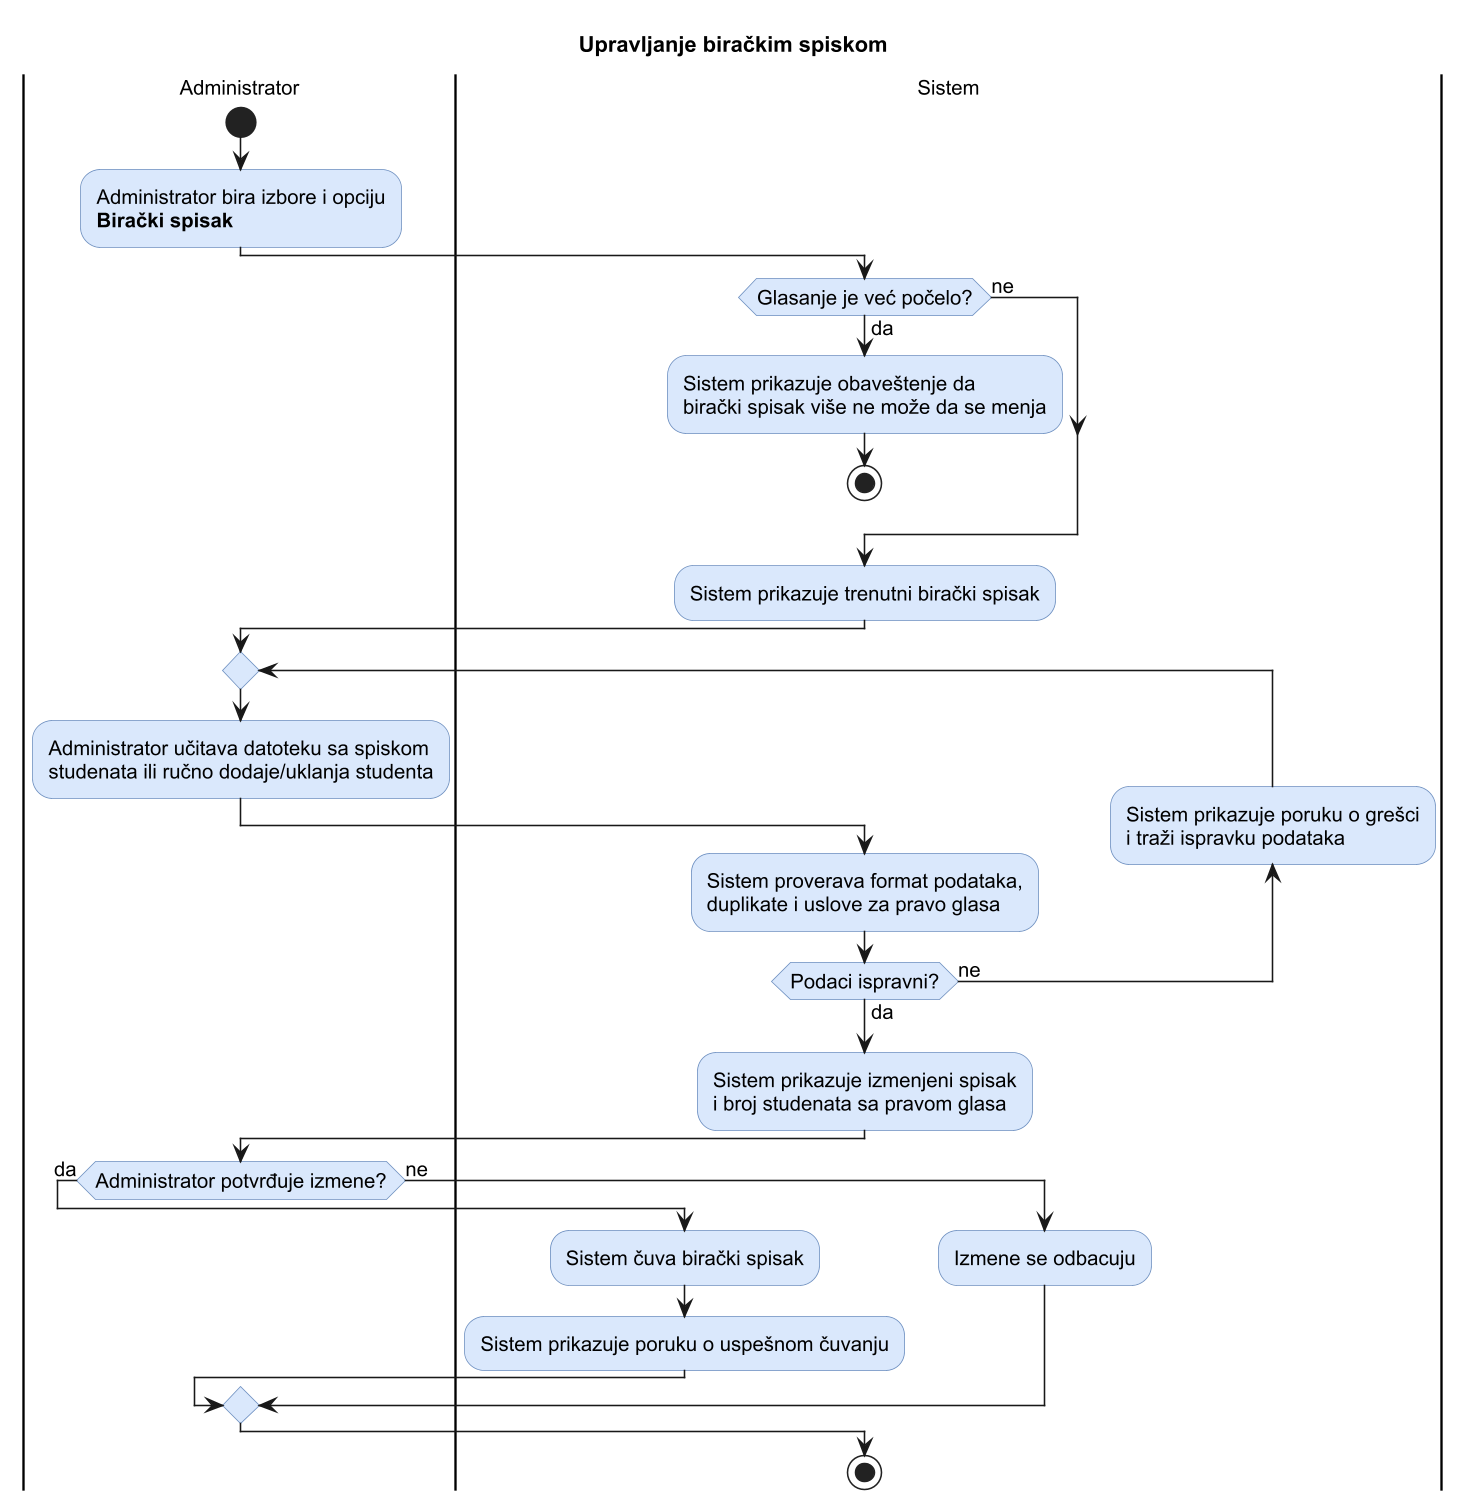
\includegraphics[width=0.85\textwidth]{aktivnosti_upravljanje_birackim_spiskom.png}
    \caption{Dijagram aktivnosti: Upravljanje biračkim spiskom}
    \label{fig:upravljanje_birackim_spiskom}
\end{figure}

\newpage
